% Options for packages loaded elsewhere
% Options for packages loaded elsewhere
\PassOptionsToPackage{unicode}{hyperref}
\PassOptionsToPackage{hyphens}{url}
\PassOptionsToPackage{dvipsnames,svgnames,x11names}{xcolor}
%
\documentclass[
  7pt,
  a4paper,
  DIV=11,
  numbers=noendperiod]{scrartcl}
\usepackage{xcolor}
\usepackage[margin=1cm,heightrounded]{geometry}
\usepackage{amsmath,amssymb}
\setcounter{secnumdepth}{-\maxdimen} % remove section numbering
\usepackage{iftex}
\ifPDFTeX
  \usepackage[T1]{fontenc}
  \usepackage[utf8]{inputenc}
  \usepackage{textcomp} % provide euro and other symbols
\else % if luatex or xetex
  \usepackage{unicode-math} % this also loads fontspec
  \defaultfontfeatures{Scale=MatchLowercase}
  \defaultfontfeatures[\rmfamily]{Ligatures=TeX,Scale=1}
\fi
\usepackage{lmodern}
\ifPDFTeX\else
  % xetex/luatex font selection
  \setmainfont[]{Inter}
\fi
% Use upquote if available, for straight quotes in verbatim environments
\IfFileExists{upquote.sty}{\usepackage{upquote}}{}
\IfFileExists{microtype.sty}{% use microtype if available
  \usepackage[]{microtype}
  \UseMicrotypeSet[protrusion]{basicmath} % disable protrusion for tt fonts
}{}
\makeatletter
\@ifundefined{KOMAClassName}{% if non-KOMA class
  \IfFileExists{parskip.sty}{%
    \usepackage{parskip}
  }{% else
    \setlength{\parindent}{0pt}
    \setlength{\parskip}{6pt plus 2pt minus 1pt}}
}{% if KOMA class
  \KOMAoptions{parskip=half}}
\makeatother
% Make \paragraph and \subparagraph free-standing
\makeatletter
\ifx\paragraph\undefined\else
  \let\oldparagraph\paragraph
  \renewcommand{\paragraph}{
    \@ifstar
      \xxxParagraphStar
      \xxxParagraphNoStar
  }
  \newcommand{\xxxParagraphStar}[1]{\oldparagraph*{#1}\mbox{}}
  \newcommand{\xxxParagraphNoStar}[1]{\oldparagraph{#1}\mbox{}}
\fi
\ifx\subparagraph\undefined\else
  \let\oldsubparagraph\subparagraph
  \renewcommand{\subparagraph}{
    \@ifstar
      \xxxSubParagraphStar
      \xxxSubParagraphNoStar
  }
  \newcommand{\xxxSubParagraphStar}[1]{\oldsubparagraph*{#1}\mbox{}}
  \newcommand{\xxxSubParagraphNoStar}[1]{\oldsubparagraph{#1}\mbox{}}
\fi
\makeatother


\usepackage{longtable,booktabs,array}
\newcounter{none} % for unnumbered tables
\usepackage{calc} % for calculating minipage widths
% Correct order of tables after \paragraph or \subparagraph
\usepackage{etoolbox}
\makeatletter
\patchcmd\longtable{\par}{\if@noskipsec\mbox{}\fi\par}{}{}
\makeatother
% Allow footnotes in longtable head/foot
\IfFileExists{footnotehyper.sty}{\usepackage{footnotehyper}}{\usepackage{footnote}}
\makesavenoteenv{longtable}
\usepackage{graphicx}
\makeatletter
\newsavebox\pandoc@box
\newcommand*\pandocbounded[1]{% scales image to fit in text height/width
  \sbox\pandoc@box{#1}%
  \Gscale@div\@tempa{\textheight}{\dimexpr\ht\pandoc@box+\dp\pandoc@box\relax}%
  \Gscale@div\@tempb{\linewidth}{\wd\pandoc@box}%
  \ifdim\@tempb\p@<\@tempa\p@\let\@tempa\@tempb\fi% select the smaller of both
  \ifdim\@tempa\p@<\p@\scalebox{\@tempa}{\usebox\pandoc@box}%
  \else\usebox{\pandoc@box}%
  \fi%
}
% Set default figure placement to htbp
\def\fps@figure{htbp}
\makeatother





\setlength{\emergencystretch}{3em} % prevent overfull lines

\providecommand{\tightlist}{%
  \setlength{\itemsep}{0pt}\setlength{\parskip}{0pt}}



 


\usepackage{wrapfig}
\usepackage{graphicx}
\makeatletter
\renewcommand{\@maketitle}{%
  \begin{center}
  \begin{minipage}[c]{0.7\textwidth}
  \raggedright
  {\LARGE \@title \par}
  \vskip 0.5em
  {\normalsize \@author \par}
  \vskip 0.3em
  {\normalsize \@date \par}
  \end{minipage}\hfill
  \begin{minipage}[c]{0.2\textwidth}
  \raggedleft
  
\includegraphics[height=1.5cm, width=\linewidth]{whanganui_council_logo.png}
  \end{minipage}
  \end{center}}
\makeatother
\KOMAoption{captions}{tableheading}
\makeatletter
\@ifpackageloaded{caption}{}{\usepackage{caption}}
\AtBeginDocument{%
\ifdefined\contentsname
  \renewcommand*\contentsname{Table of contents}
\else
  \newcommand\contentsname{Table of contents}
\fi
\ifdefined\listfigurename
  \renewcommand*\listfigurename{List of Figures}
\else
  \newcommand\listfigurename{List of Figures}
\fi
\ifdefined\listtablename
  \renewcommand*\listtablename{List of Tables}
\else
  \newcommand\listtablename{List of Tables}
\fi
\ifdefined\figurename
  \renewcommand*\figurename{Figure}
\else
  \newcommand\figurename{Figure}
\fi
\ifdefined\tablename
  \renewcommand*\tablename{Table}
\else
  \newcommand\tablename{Table}
\fi
}
\@ifpackageloaded{float}{}{\usepackage{float}}
\floatstyle{ruled}
\@ifundefined{c@chapter}{\newfloat{codelisting}{h}{lop}}{\newfloat{codelisting}{h}{lop}[chapter]}
\floatname{codelisting}{Listing}
\newcommand*\listoflistings{\listof{codelisting}{List of Listings}}
\makeatother
\makeatletter
\makeatother
\makeatletter
\@ifpackageloaded{caption}{}{\usepackage{caption}}
\@ifpackageloaded{subcaption}{}{\usepackage{subcaption}}
\makeatother
\usepackage{bookmark}
\IfFileExists{xurl.sty}{\usepackage{xurl}}{} % add URL line breaks if available
\urlstyle{same}
\hypersetup{
  pdftitle={Are rates fair?},
  pdfauthor={John Lavack, 20001249},
  colorlinks=true,
  linkcolor={blue},
  filecolor={Maroon},
  citecolor={Blue},
  urlcolor={Blue},
  pdfcreator={LaTeX via pandoc}}


\title{Are rates fair?}
\author{John Lavack, 20001249}
\date{2026-10-18}
\begin{document}
\maketitle


Residential rate payers make up 88.4\% of rateable units and 77\% of
total rate income. The majority of the rate burden falls on them. Which
raises discussion around whether rates are `fair'. This analysis asks
whether Whanganui residential rates are distributed proportionally to
property value, and if not, what mechanisms drive the deviation. For
this analysis residential rates refers to both residential and lifestyle
QV categories.

The following analysis uses Whanganui Council rates from 2022 to 2026
only. Total rates are analysed, these are comprised of fixed and
variable portions. For the purpose of this analysis separating the fixed
rate component was done using draft rates by property for 26/27.

Let's start with\ldots{}

\pandocbounded{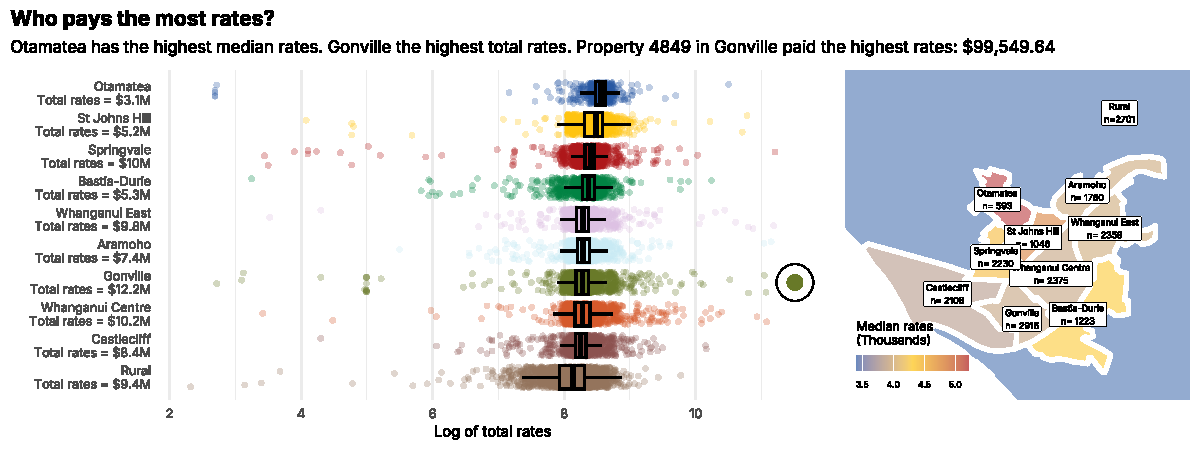
\includegraphics[keepaspectratio]{project_20001249_files/figure-pdf/graph 1 and 2 output-1.pdf}}

The answer depends on the unit of analysis. Individually, the owner of
property 4849 in Gonville paid the most rates in 2026. By suburb,
Otamatea ratepayers pay the highest median (\$5,213) but, as a group,
contributed the least in total (\$3.1 million) --- there only 593.
Gonville, with a lower median (\$3,928), has the most ratepayers (2,701)
and contributes more in aggregate. Suburb size doesn't map directly to
total rates because housing density is independent of area. The box plot
below shows the log of rates to accommodate the many outliers within
each suburb.

Rates are not evenly distributed, and neither are people.

\pandocbounded{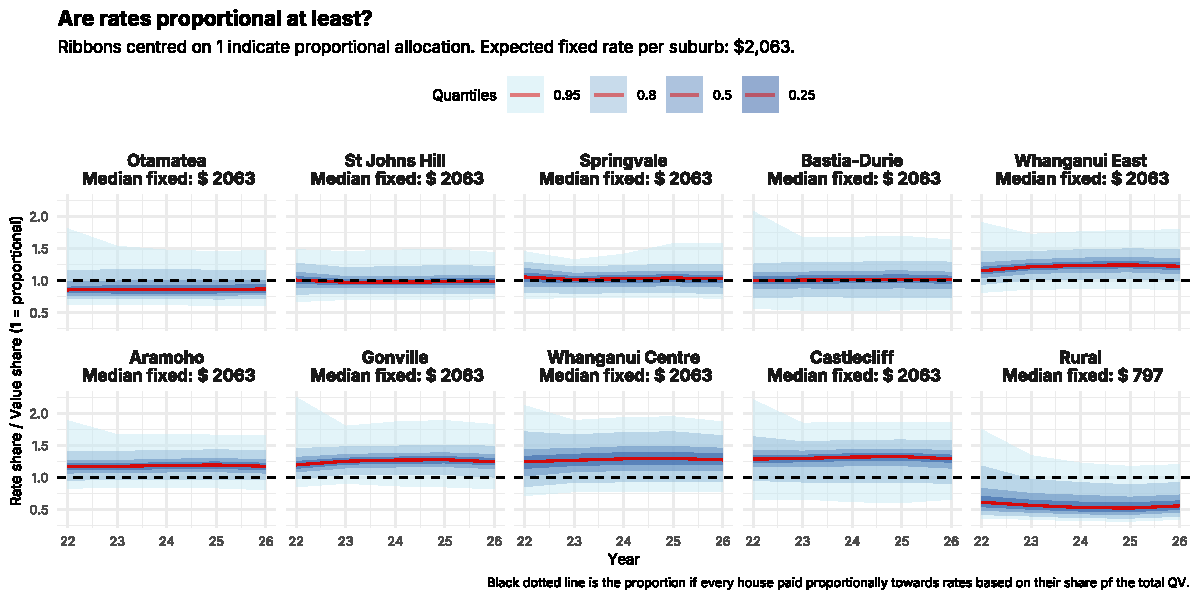
\includegraphics[keepaspectratio]{project_20001249_files/figure-pdf/graph 3 output-1.pdf}}

If rates were allocated purely by property value --- ``each household is
rated according to the value of their property'' (Whanganui City
Council, 2026) --- then each suburb's share of the total rate bill
should equal its share of total QV. The proportional plot tests this: a
suburb on the dashed line is paying exactly its QV-proportional share.

It's not that simple, because rates are a combination of a fixed
per-property charge and a proportional charge linked to QV
(calculate.co.nz, 2026). The fixed value is the same dollar amount per
SUIP regardless of property value, \$2,063, so it weighs more heavily on
lower-QV properties and less on higher-QV ones. This single mechanism
explains most of the deviation from the proportional line:

\begin{itemize}
\tightlist
\item
  St Johns Hill, Springvale, Bastia-Durie sit on or near the line ---
  their QV and density happen to balance out.
\item
  Otamatea sits slightly below. Its high median QV means the fixed
  amount is a small fraction of each bill (\$2,010), pulling the suburb
  below the line. In absolute terms it pays the most; proportionally,
  it's underpaying.
\item
  Rural sits well below. With 2,701 units (second most in the city) and
  large land holdings (recall the map above), the fixed amount is a tiny
  fraction of each bill, only \$1,021, about half of every other suburb.
  Rural also pays roughly half of what a pure QV-proportional system
  would predict.
\item
  Whanganui East, Centre, Aramoho, Gonville, Castlecliff sit above.
  Their moderate QV means the fixed portion is a larger fraction of each
  bill, pushing them above the line. Castlecliff has few high outliers
  and still sits above, ruling out outliers as the explanation for
  proportionality. However, due to these outliers, their fixed portions
  are higher than the expected amount.
\end{itemize}

\begin{quote}
Note: the mean fixed rate is shown per suburb, as this shows the impact
of outliers
\end{quote}

So paying the most in dollars is not the same as paying
disproportionately. Otamatea's high rates are a direct consequence of
its high property values. The suburbs that are overpaying relative to
their QV share are the mid-value, higher-density ones --- a density
penalty.

\pandocbounded{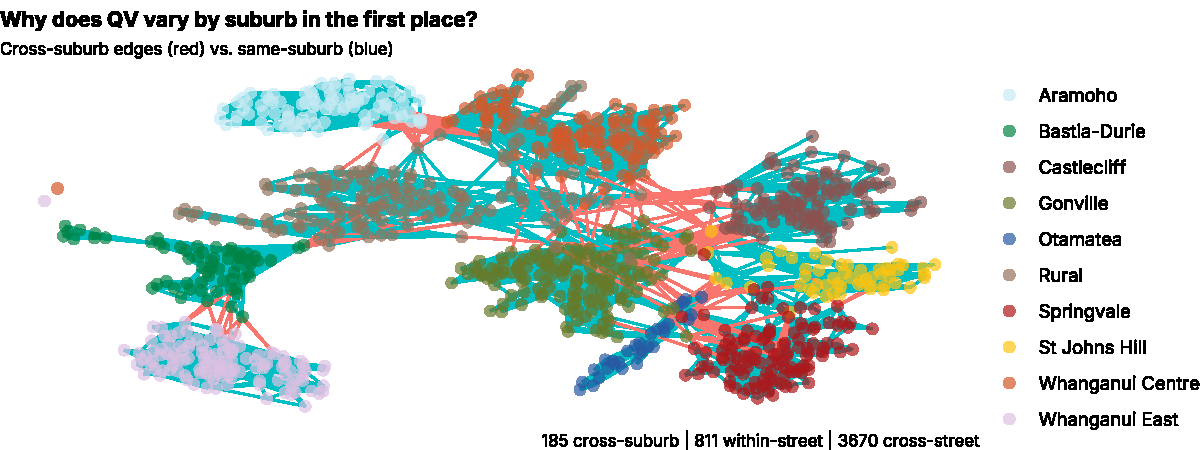
\includegraphics[keepaspectratio]{project_20001249_files/figure-pdf/graph 5 output-1.pdf}}

The proportional plot shows how rates deviate from QV proportionality.
But it doesn't explain why QV itself is so suburb-specific. If QV were
driven primarily by property characteristics --- size, age, land area
--- we'd expect similar houses in different suburbs to have similar QVs.
The network plot (a force directed network, with k-nearest-neighbour
similarity, k=3), proportional share decomposition.tests this. It
connects each property to its three closest QV neighbours (many more and
the plot would be unreadable) and shows where they fall. In the plot
below, QV value calculated as \(QV = CV + LV + (CV - LV)\) (QV, 2026).

In the proportional 997-unit sample below, 96\% of each property's top-3
QV neighbours are in the same suburb. Only 4\% cross a suburb boundary.
The similarity is strongest within a suburb but not specifically within
a street. QV clustering operates at the suburb scale, not the street
scale.

This means QV is set by location, not by the house itself. Two identical
houses in different suburbs will have different QVs because the local
market; demand, amenities, distance from CBD, school catchments, etc ---
sets the QV. A desirability premium that tracks the suburb's market
position, not the property's physical attributes.

\section{Two premiums, one bill}\label{two-premiums-one-bill}

The rate bill is shaped by two distinct mechanisms:

\begin{itemize}
\item
  A density premium, a fixed amount effect. Fixed per-property charges
  are a larger fraction of the bill in moderate-QV, high-density suburbs
  and a smaller fraction in high-QV, low-density areas (rural,
  Otamatea). This pushes dense suburbs above the proportional line and
  less dense ones below it.
\item
  A desirability premium, the QV effect. QV is set at the suburb level
  by the local market. Suburbs in higher demand have higher QV's across
  the board, which raises the proportional component of every rate bill
  in that suburb.

  Taken together they mean the ``each household pays according to
  value'' statement is an oversimplification. The rate bill is shaped by
  where you live, how many neighbours share the fixed charges, and what
  the local market is willing to pay for that location.
\end{itemize}

\section{So, are rates fair?}\label{so-are-rates-fair}

That depends on what ``fair'' means. If fairness means ``your share of
the bill equals your share of property value,'' then no --- the fixed
portion alone breaks that.\\
If fairness means ``people in the same suburb pay the same rate,'' then,
after accounting for outliers, yes.\\
If fairness means ``you pay for what you use,'' then the fixed amount is
regressive and the QV component is not.

The data doesn't answer the question. It shows the mechanism. Whether
the mechanism is fair is a question for the ratepayers.

========================

\section{References:}\label{references}

\begin{enumerate}
\def\labelenumi{\arabic{enumi}.}
\item
  Calculate.co.nz. (2026). \emph{How Are Council Rates Calculated in NZ
  \textbar{} Capital Value Explained}.
  https://www.calculate.co.nz/learning-center/council-rates-guide.php
\item
  QV. (2026). \emph{Understanding your rating value}.
  https://content.quotablevalue.co.nz/media/documents/QV\_Understanding\_Rating\_Values\_Guide.pdf
\item
  Whanganui Council. (2026). \emph{Rates}.
  https://www.whanganui.govt.nz/Property-and-Rates/Rates
\end{enumerate}




\end{document}
